%%% In this section, you will describe all of the various artifacts that you will generate and maintain during the project life cycle. Describe the purpose of each item below, how the content will be generated, where it will be stored, how often it will be updated, etc. Replace the default text for each section with your own description. Reword this paragraph as appropriate.

\subsection{Major Documentation Deliverables}
\subsubsection{Project Charter}
This document will only be updated when or if there are any changes in our vision, mission, success criteria, system overview, roles, budget, equipment, facilities, constraints, or risks. We plan on delivering our initial version on Tuesday October 1, 2019. The final version will be delivered the last week of class.
\subsubsection{System Requirements Specification}
The system requirements document will be started once we figure out all of our system requirements and if anything changes we will update the document accordingly.  The initial version will be delivered on October 22, 2019 and the final version will be submitted the last week of class.

\subsubsection{Architectural Design Specification}
The Architectural design specification document initial version will be delivered November 12, 2019 and the final version will be submitted the last week of class. The document will be updated as needed, meaning if there are any changes in the architectural design this includes the finest details.

\subsubsection{Detailed Design Specification}
The Detailed Design specification document initial version will be delivered on December 2, 2019 and this will be the final version. We assume the document will not need any updating we plan on having all aspects of the project in order.

\subsection{Recurring Sprint Items}
The following items will be documented and maintained during each individual sprint. As above, remove this paragraph from your draft, but leave the heading.

\subsubsection{Product Backlog}
Items will be added to the product backlog as we work through the previous requirements and then get to the new requirements. All SRS items will go through thorough analysis before being added to the product backlog, to gain a full understanding of all customer needs .Item prioritization will be done by the team lead and will be prioritized by which items needs immediate attention. Product backlog will be shared and updated through Google Drive.

\subsubsection{Sprint Planning}
How will each sprint plan be planned? How many sprints will there be (you need to look at the schedules for this course and previous Senior Design II courses during the appropriate semesters to figure this out).

\subsubsection{Sprint Goal}
The team lead ultimately decides the sprint goal, but sprint goals are suggested by the entire team including the customer. Sprint goals will go through thorough analysis before being added. The customer will be either on call or in person when going over the sprint goals.

\subsubsection{Sprint Backlog}
Team lead will decide which product backlog items make their way into the sprint backlog, after informing the team and getting everyone's perspective on the task. The document will be maintained on Google Sheets. 

\subsubsection{Task Breakdown}
Tasked will be assigned by team members volunteering to claim a task. In order to document the time spent on a task will be through a time in time out portion on excel. Team members will enter the time they started a task and stop a task each day, then we will calculate the hours spent on the task. This will be in the scrum excel file.

\subsubsection{Sprint Burn Down Charts}
Who will be responsible for generating the burn down charts for each sprint? How will they be able to access the total amount of effort expended by each individual team member? What format will the burn down chart use (include an example burn down chart below).

\begin{figure}[h!]
    \centering
    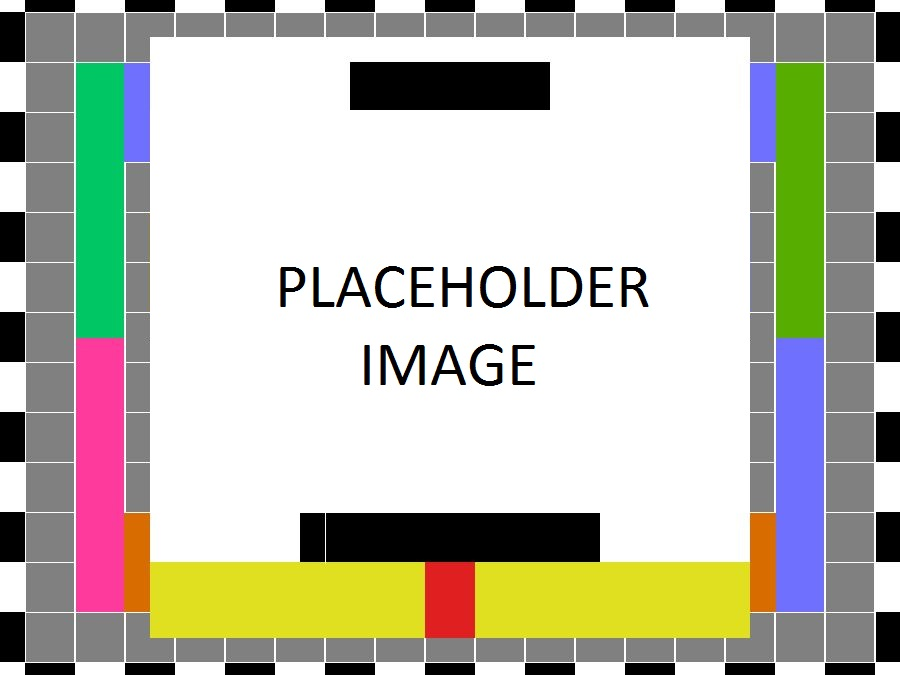
\includegraphics[width=0.5\textwidth]{images/test_image}
    \caption{Example sprint burn down chart}
\end{figure}

\subsubsection{Sprint Retrospective}
How will the sprint retrospective be handled as a team? When will this discussion happen after each sprint? What will be documented as a group and as individuals, and when will it be due?

\subsubsection{Individual Status Reports}
What sort of status will be reported by each individual member, and how often will it be reported? What key items will be contained in the report?

\subsubsection{Engineering Notebooks}
How often will the engineering notebook be updated, at a minimum, by each team member? What is the minimum amount of pages that will be completed for each interval, and how long will that interval be? How will the team keep each member accountable? Who will sign of as a "witness" for each ENB page?

\subsection{Closeout Materials}
The following materials, in addition to major documentation deliverables, will be provided to the customer upon project closeout. Remove this paragraph from your draft, but leave the heading.

\subsubsection{System Prototype}
What will be included in the final system prototype? How and when will this be demonstrated? Will there be a Prototype Acceptance Test (PAT) with your customer? Will anything be demonstrated off-site? If so, will there be a Field Acceptance Test (FAT)?

\subsubsection{Project Poster}
What will be included on the poster, what will be the final dimensions, and when will it be delivered?

\subsubsection{Web Page}
What will be included on the project web page? Will it be accessible to the public? When will this be delivered? Will it be updated throughout the project, or just provided at closeout (at a minimum, you need to provide a simple web page at the end).

\subsubsection{Demo Video}
What will be shown in the demo video(s)? Will you include a B-reel footage for future video cuts? Approximately how long will the video(s) be, and what topics will be covered?

\subsubsection{Source Code}
How will your source code be maintained? What version control system will you adopt? Will source code be provided to the customer, or binaries only? If source code is provided, how will it be turned over to the customer? Will the project be open sourced to the general public? If so, what are the license terms (GNU, GPL, MIT, etc.). Where will the license terms be listed (in each source file, in a single readme file, etc.).

\subsubsection{Source Code Documentation}
What documentation standards will be employed? Will you use tools to generate the documentation (Doxygen, Javadocs, etc.). In what format will the final documentation be provided (PDF, browsable HTML, etc.)?

\subsubsection{Hardware Schematics}
Will you be creating printed circuit boards (PCBs) or wiring components together? If so, list each applicable schematic and what sort of data it will contain (PCB layout, wiring diagram, etc.). If your project is purely software, omit this section.

\subsubsection{CAD files}
Will the project involve any mechanical design, such as 3D printed or laser-cut parts? If so, what software will you use to generate the files and what file formats will you provide in your closeout materials (STL, STEP, OBJ, etc.). If your project is purely software, omit this section.

\subsubsection{Installation Scripts}
How will the customer deploy software to new installations? Will you provide installation scripts, install programs, or any other tools to improve the process? Will there be multiple scripts provided (perhaps separate scripts for the graphical front end and back end server software)? 

\subsubsection{User Manual}
Will you customer need a printed or digital user manual? Will they need a setup video? Decide now what will be provided and discuss.
